%!TEX program = xelatex
\documentclass[12pt]{article}
\usepackage{amsmath}
\usepackage[usenames,dvipsnames,svgnames,table]{xcolor}
\usepackage[colorlinks=true,urlcolor=blue,linkcolor=blue]{hyperref}
\usepackage{graphicx}
\usepackage{titlesec}
\usepackage[raggedright]{sidecap}
\sidecaptionvpos{figure}{c}
\usepackage{ifxetex}
\ifxetex
\usepackage{mathspec}
\usepackage{xunicode}
\defaultfontfeatures{Mapping=tex-text}
\defaultfontfeatures{Ligatures=TeX}
% \setromanfont{Iowan Old Style Roman}
\setsansfont{PT Sans}
% \setmathfont{XITS Math}
% \setmathrm{XITS Math}
\setmonofont[Scale=0.8]{Menlo}
\else
\usepackage[utf8]{inputenc}
\usepackage[T1]{fontenc}
\fi

% Section header formatting
\titleformat{\section}
  {\normalfont\sffamily\Large\bfseries\color{DarkSlateBlue}}
  {\thesection}{1em}{}
\titleformat{\subsection}
  {\normalfont\sffamily\large\bfseries\color{SteelBlue}}
  {\thesubsection}{1em}{}

% Commands, aliases, etc
\graphicspath{{./figs/}{./}}
\newcommand{\xvec}{\mathbf{x}}
\newcommand{\rvec}{\mathbf{R}}
\newcommand{\thetavec}{\mathbf{\theta}}
\newcommand{\prior}{P(\thetavec)}
\newcommand{\post}{P(\thetavec|\xvec)}
\newcommand{\like}{P(\xvec|\thetavec)}
\newcommand{\ilike}{P(\xvec_i|\thetavec)}
\newcommand{\data}{\{\xvec_i\}_{i=1}^m}
\newcommand{\eptdata}{\xvec^{\mathrm{Y}}}
\newcommand{\dcadata}{\xvec^{\mathrm{D}}_j}


\title{\sffamily\bfseries{Appendix on electron unfolding for PRC manuscript}}
\author{\sffamily{Andrew Adare}}
% \author{\fontspec{Helvetica Neue}{Andrew Adare, Darren McGlinchey, Jin Huang}}
\date{\sffamily{\today}}
\begin{document}
\maketitle

\section{Appendix: electron unfolding}

\subsection{Introduction}
The unfolding problem involves inferring the invariant yields of charm and beauty parent hadrons from the observed nonphotonic electron distributions. There are many unfolding algorithms that could be applied to this end, but Bayesian unfolding techniques~\cite{Choudalakis:2012hz} have the important advantage of providing a joint probability density over the model parameters, which are in this case the set of parent hadron yields within each $p_T$ interval. This is in principle the entirety of the available information, in constrast to techniques involving maximum likelihood estimation (MLE) or maximum a posteriori (MAP) estimation which can at best compute only the first two moments of the posterior distribution.

Our unfolding method uses the generative approach of modeling a likelihood function and using Bayes' rule to compute the posterior from the likelihood and prior information. This can be contrasted with discriminative approaches, which directly compute estimates of the posterior by optimizing model parameters to the fit the data.

The method specifically involves sampling from the posterior using a
Markov Chain Monte Carlo (MCMC) algorithm, which makes accurate sampling of multidimensional distributions far more efficient than uniform sampling. The MCMC variant used here is an affine-invariant ensemble sampler developed in~\cite{goodman2010} and implemented in~\cite{dfm2013}. It is well-suited to distributions that are highly anisotropic such as spectra which often vary over many orders of magnitude.

\subsection{Decay model and matrix normalization}
The Pythia generator was used to generate parent hadrons. TODO (Darren): Number of events, pythia version and settings, PID selection, kinematic cuts, acceptance cuts, any other details.

The probability for a charm or beauty hadron at a given $p_T$ to decay to an electron at a given $p_T$ (and DCA) is encoded in a matrix whose rows are measurements (e.g. electron $p_T$) and whose columns are intervals in parent hadron $p_T$. Some examples are shown in figure~\ref{fig:mat}.
\begin{figure}[tb]
  \begin{center}
    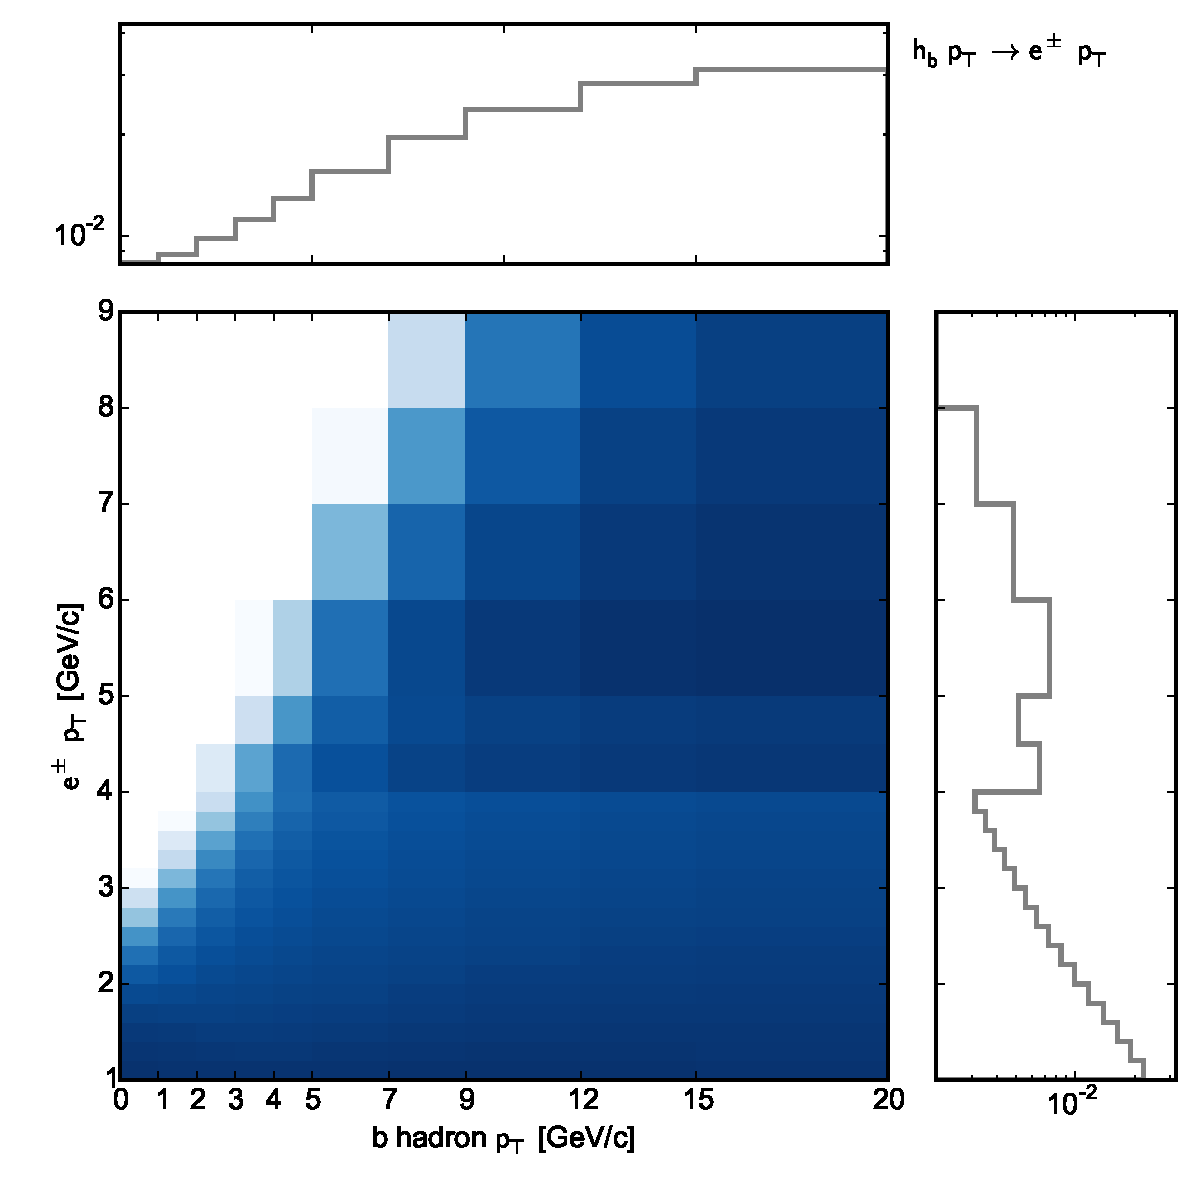
\includegraphics[width=0.48\textwidth]{eptmat_b}
    \quad
    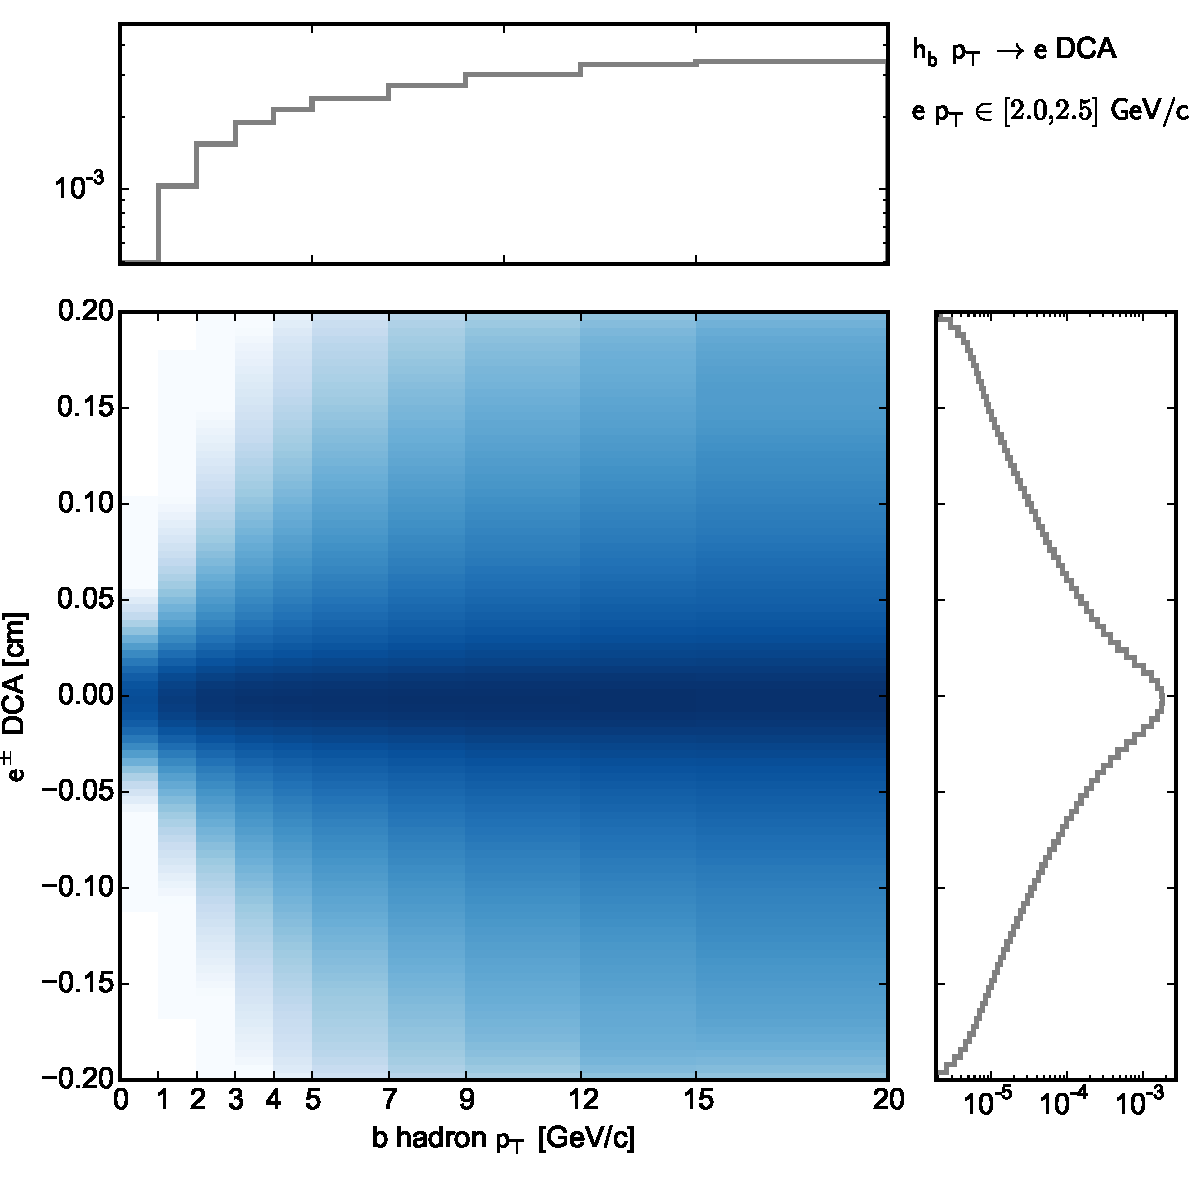
\includegraphics[width=0.48\textwidth]{dcamat_b_2}
  \end{center}
  \caption{Examples of decay matrices produced from pythia events. Left: decay probabilities for b hadrons to electron $p_T$. Right: decay probabilities for b hadrons to electron DCA for electrons in the 2.0-2.5 GeV/$c$ $p_T$ range. The top and side panels show the univariate marginal probability distributions.}
  \label{fig:mat}
\end{figure}

Note that the marginal probabilities do not integrate to unity in these matrices. This is because the decay probabilities are normalized to the number of hadrons that are generated at all momenta and in all directions (see figure~\ref{fig:gen}).
\begin{figure}[tb]
  \begin{center}
    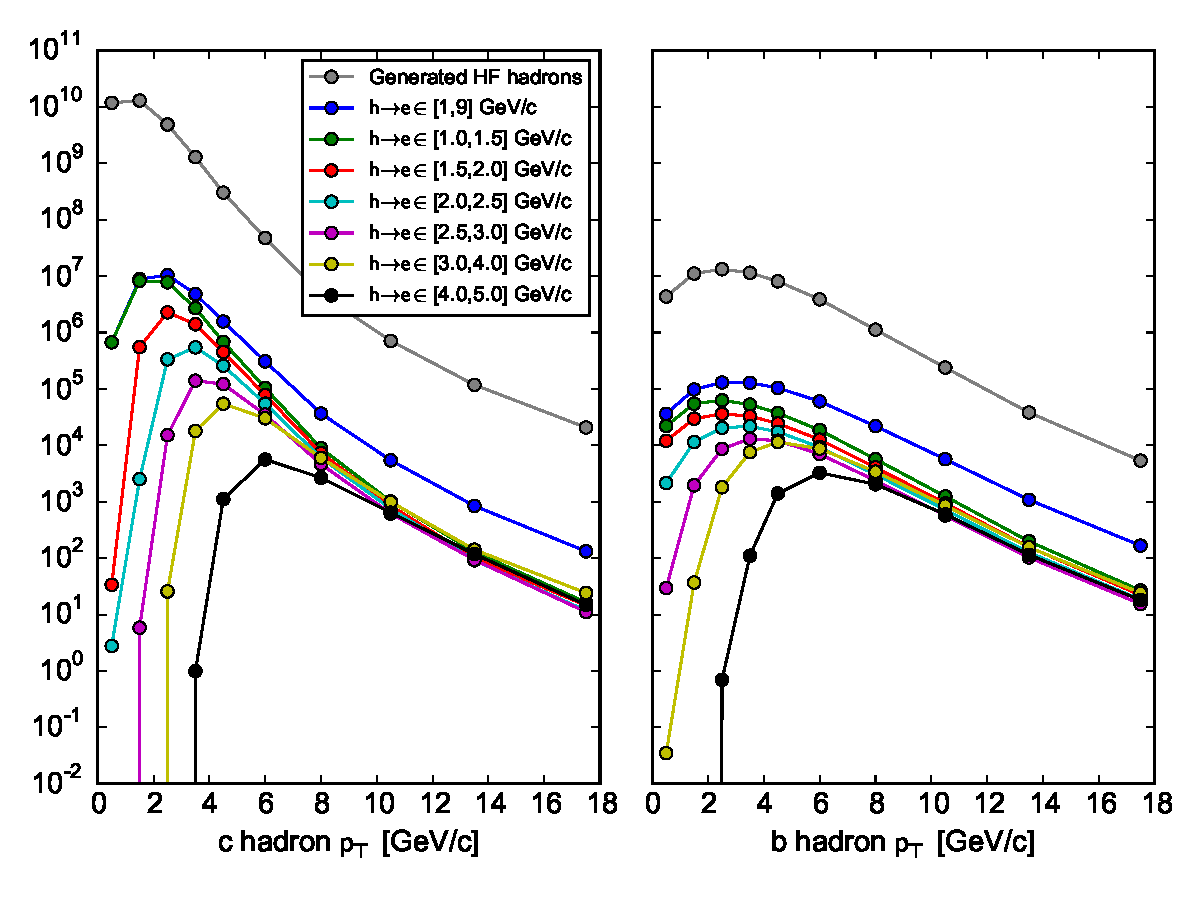
\includegraphics[width=0.98\textwidth]{hpt-gen}
  \end{center}
  \caption{Transverse momentum of c and b hadrons as generated by pythia. The gray points represent all generated hadrons; the colored points represent hadrons falling within the specified $p_T$ intervals. The columns of each decay matrix is divided by the gray distribution to represent the decay probabilities.}
  \label{fig:gen}
\end{figure}


\subsection{Likelihood function}
The goal is to evaluate the likelihood $\ilike$ for each of $m$ measurements in the dataset $\data$ which, along with prior information $\prior$, can be used to compute the posterior density $\post$ over invariant yields in each parent hadron $p_T$ bin, here, denoted $\theta$:
\begin{equation}\label{eq:bayesrule}
  \post = \frac{\prod_{i=1}^m \ilike \prior}{P(\xvec_{1\ldots m})}.
\end{equation}

This analysis is based on a dataset composed of electron invariant yield points $\eptdata$ and six electron DCA distributions $\dcadata$, where $j$ signifies each electron $p_T$ interval.

The $\eptdata$ dataset has been corrected for background, efficiency, and acceptance, and has been assigned statistical uncertainties that are assumed to be normally distributed and uncorrelated. Thus, the likelihood for $\eptdata$ is modeled as a multivariate Gaussian with diagonal covariance.

The DCA datasets, in contrast, each consist of a histogrammed distribution of integer-valued entries, and are thus more appropriately described by a multivariate Poisson distribution.

As is customary, the logarithm of the likelihood function is used in practice. The combined (log) likelihood for the data is explicitly
\begin{equation} \label{eq:logl}
  \ln \like = \ln P(\eptdata|\thetavec) + \sum_{j=1}^6 \ln P(\dcadata|\thetavec)
\end{equation}
where
\begin{equation} \label{eq:llgauss}
  \ln \like = -\frac{m \log 2\pi}{2} - \frac{m \log \sigma^2}{2} - \frac{1}{2} (\xvec - M \thetavec)^T \Sigma^{-1} (\xvec - M \thetavec) 
\end{equation}
and
\begin{equation} \label{eq:llpoiss}
  TODO
\end{equation}

\subsection{Initialization} \label{sec:mcmc-init}
The ensemble of 500 Markov Chains or ``walkers'' is initialized around the value of $\thetavec$ generated by pythia. This starting point, $\thetavec_{\mathrm{ini}}$, is shown as the grey curve in figure~\ref{fig:gen}. The walkers are distributed randomly according to a normal distribution centered at $\thetavec_{\mathrm{ini}}$ with $\sigma = 0.1 \thetavec_{\mathrm{ini}}$.

\subsection{Regularization/prior}
Information that is external to the dataset itself is included by adding a term to the right hand side of equation~\ref{eq:logl}. In this analysis we included a squared-exponential function
\begin{equation} \label{eq:l2reg}
  \ln \prior = -\alpha^2 \left(||L \rvec_c||_2^2 + ||L \rvec_b||_2^2\right)
\end{equation}
where $\rvec_c$ and $\rvec_b$ are ratios of the charm and beauty components of the parent hadron $p_T$ vector to the corresponding components of $\thetavec_{\mathrm{ini}}$, and $L$ is an $N$-by-$N$ second-order finite-difference matrix of the form
\begin{equation} \label{eq:lmatrix}
L = \frac{N}{2}
\begin{pmatrix}
-1 & 1 & & & & & &\\
1 & -2 & 1 & & & & &\\
& 1 & -2 & 1 & & & &\\

& & \ddots & \ddots & \ddots & & & &\\
% & & & & & & & & \\
& & & \ddots & \ddots & \ddots & & & \\
% & & & & & & & & \\

& & & & 1 & -2 & 1 &\\
& & & & & 1 & -2 & 1\\
& & & & & & 1 & -1
\end{pmatrix}.
\end{equation}
Thus the addition of this term encodes the assumption that departures from the pythia model should be smooth by penalizing total curvature as measured by the second derivative. $\alpha$ is a regularization hyperparameter set to 0.2 for this analysis.

\subsection{Solution envelope, iteration schedule, and convergence}
In addition to the smoothness requirement imposed by regularization, the sampling volume is bounded in the interval $[0.001, 5] \cdot \thetavec_{\mathrm{ini}}$, which is chosen to be conservative, but speeds convergence by limiting random excursions to regions that are unrealistically far from the solution.

The sampling algorithm is first run using the initialization scheme described in~\ref{sec:mcmc-init}, and a burn-in period of 1000 steps is passed before storing samples. If the burn-in period is not sufficiently long, the posterior probability over all the walkers will indicate a net increase over time, as shown in the left side of figure~\ref{fig:timeseries}.
\begin{figure}[tb]
  \begin{center}
    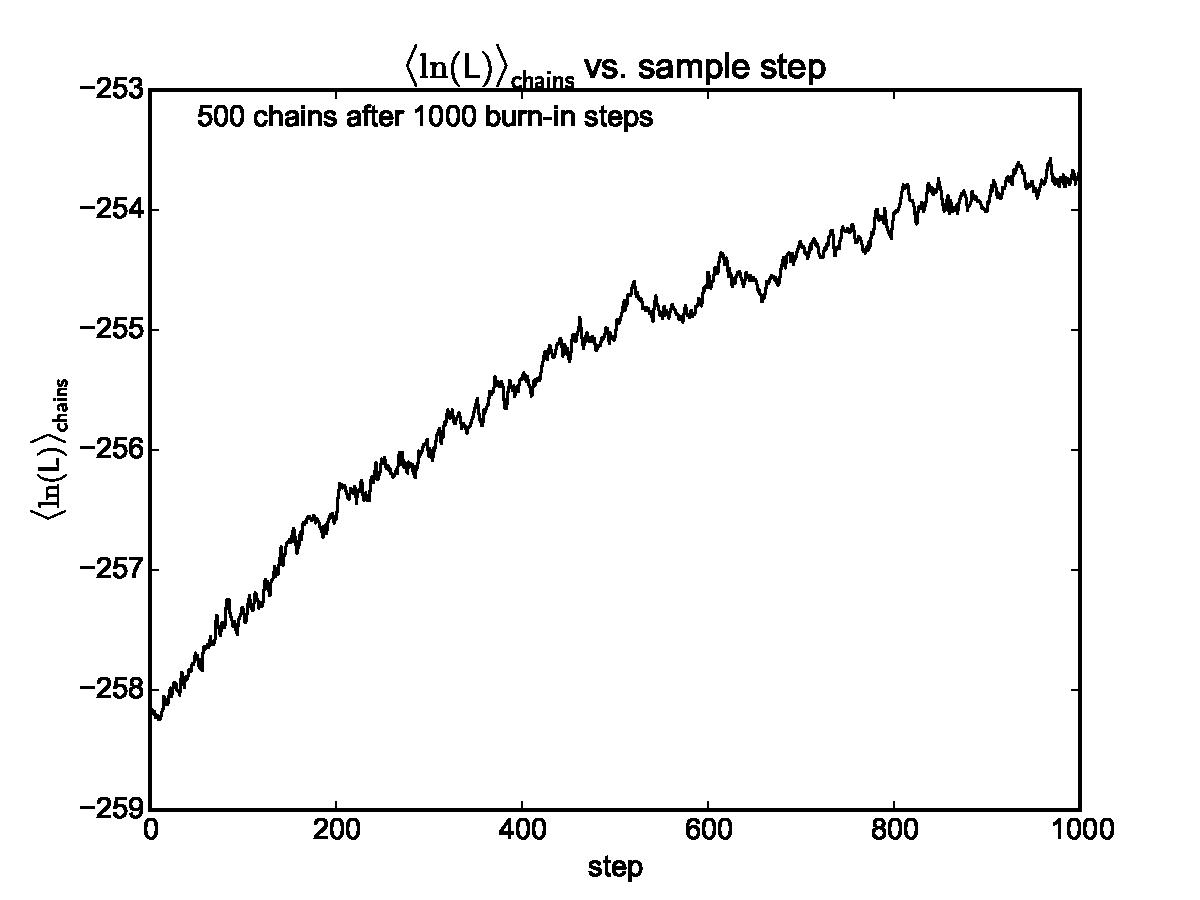
\includegraphics[width=0.48\textwidth]{AuAu200MB/1/lnprob-vs-step}
    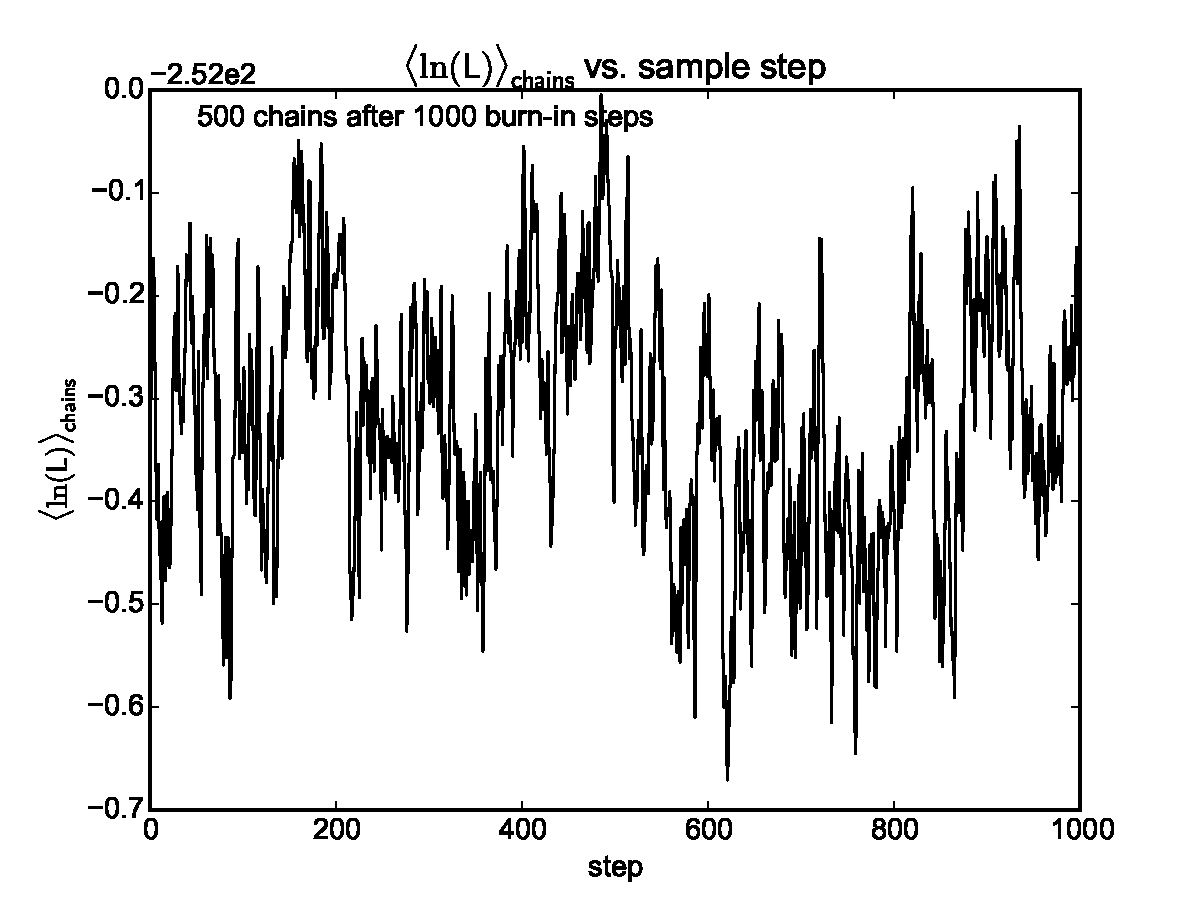
\includegraphics[width=0.48\textwidth]{AuAu200MB/2/lnprob-vs-step}
  \end{center}
  \caption{Mean log posterior probability over walkers as a function of recorded sampling step. Left: first sampling run, where chains have not fully converged to the maxim-posterior region, and the likelihood is still increasing. Right: second run initialized around the result of the first run. After the chains have drifted to the neighborhood of maximum probability, changes in the posterior probability are dominated by random fluctuations and trend over many timesteps is flat. TODO replace figures to say P or prob instead of L}
  \label{fig:timeseries}
\end{figure}
The second sampling run is initialized using the results of the first, and the sampling boundary is adjusted accordingly. This time, the parameters begin significantly closer to their optimal values, and after a similar burn-in period of discarded samples, they have drifted to regions of maximal probability and a time series of the mean likelihood shows no long-term increase.

\subsection{Posterior marginalization and statistical uncertainty}
The outcome of the sampling process is the full joint posterior density $\post$ which is 20 dimensional in this case. A univariate marginal density for each $p_T$ interval is shown in figure~\ref{fig:post}.
\begin{figure}[tb]
  \begin{center}
    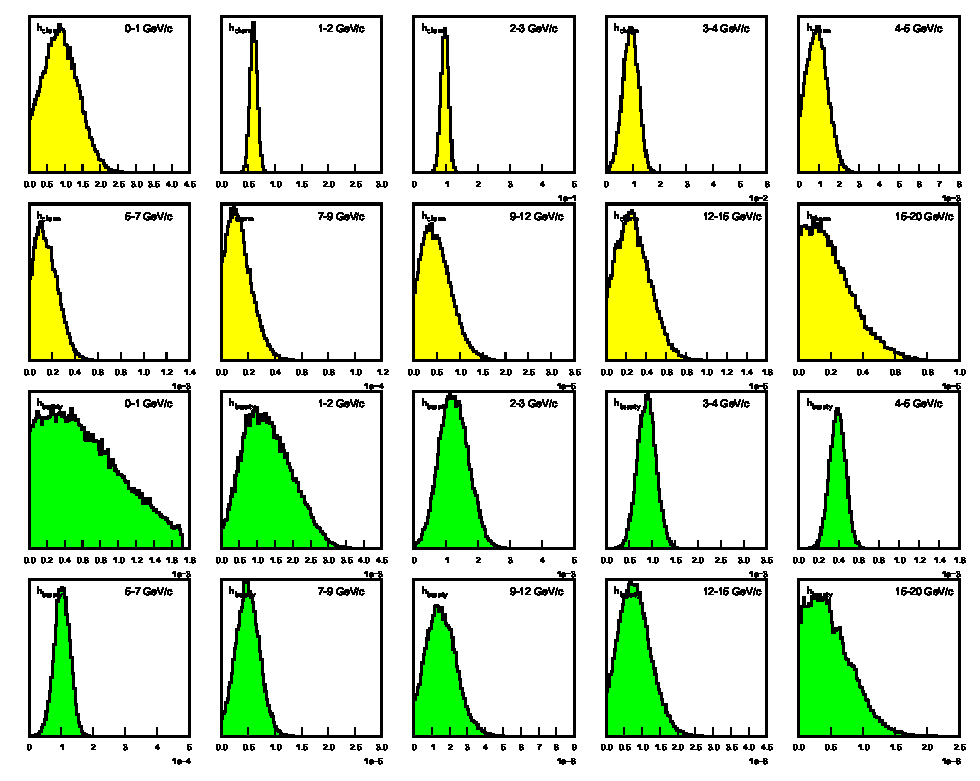
\includegraphics[width=0.98\textwidth]{AuAu200MB/2/posterior}
  \end{center}
  \caption{Marginal distributions from the sampled posterior density. Top: charm hadron pt bins. Bottom: beauty hadron pt bins.}
  \label{fig:post}
\end{figure}
TODO: show triangle plot including 2d distributions of off-diagonal parameter pairs?

\subsection{Re-fold cross-checks}
TODO
\subsection{Computing the b fraction}
TODO

%%%%%%%%%%%%%%%%%%%%%%%%%%%%%%%%%%%%%%%%%%%%%%%%%%%%%%%%%%%%%%%%%%%%%%%%%%%%%%%

\begin{thebibliography}{99}
\bibitem{Choudalakis:2012hz} 
  G.~Choudalakis,
  ``Fully Bayesian Unfolding,''
  arXiv:1201.4612 [physics.data-an].
  %%CITATION = ARXIV:1201.4612;%%
  %11 citations counted in INSPIRE as of 22 Dec 2014

\bibitem{goodman2010}
  Jonathan Goodman and Jonathan Weare,
  ``Ensemble samplers with affine invariance'',
  Communications in Applied Mathematics and Computer Science,
  Vol. 5 (2010), No. 1, 65–80.

\bibitem{dfm2013}
Foreman-Mackey, D. and Hogg, D.~W. and {Lang}, D. and {Goodman}, J.,
``emcee: The MCMC Hammer'',
Publications of the Astronomical Society of the Pacific, Volume 125, issue 925, pp.306-312.
% @ARTICLE{2013PASP..125..306F,
%    author = {{Foreman-Mackey}, D. and {Hogg}, D.~W. and {Lang}, D. and {Goodman}, J.
%   },
%     title = "{emcee: The MCMC Hammer}",
%   journal = {\pasp},
% archivePrefix = "arXiv",
%    eprint = {1202.3665},
%  primaryClass = "astro-ph.IM",
%  keywords = {Data Analysis and Techniques},
%      year = 2013,
%     month = mar,
%    volume = 125,
%     pages = {306-312},
%       doi = {10.1086/670067},
%    adsurl = {http://adsabs.harvard.edu/abs/2013PASP..125..306F},
%   adsnote = {Provided by the SAO/NASA Astrophysics Data System}
% }


\end{thebibliography}
\end{document}
